\section{Theoretical Framework}

% TODO: Humanise
\subsection{Prediction Markets} \label{sec:prediction_markets}

Prediction markets are financial markets designed to forecast future events. Participants of prediction markets trade state-contingent claims whose payoff depends on how those future events unfold.
While different types of prediction markets have been designed, the scope of this thesis is limited to winner-take-all prediction markets. These markets are typically structured in the following way: a claim costs $\$p$ today and pays $\$1$ if and only if the stated event occurs, and $\$0$ otherwise. This structure implies two participants agreeing on the price $\$p$ which one of the participants pays, the other putting up $\$(1 - p)$, with the winner receiving "all" of the dollar put up in collateral as their payoff. \citep{wolfers_prediction_2004}. 
% Arrow-Debreu securities? 
% The price $p$ can be read as the market-implied (risk-neutral) probability that the event happens, because the contract’s expected payoff equals p. Put differently, the price is a state price; under standard assumptions it coincides with the event’s probability. The same logic underlies families of related contracts (for example, across thresholds or outcomes), whose internal consistency and co-movement reflect how new information is incorporated through trading.

Through price discovery, traditional financial markets aggregate information about the value of assets. Prediction markets’ primary purpose is leveraging this role of markets for forecasting. Under the Efficient Markets Hypothesis, the market price on prediction markets should reflect the risk-neutral probabilities of the event in question, encompassing all available information.
\citep{berg_prediction_2008}


% A winner-take-all example makes this concrete. Suppose there is a market on an election between two candidates, A and B. The contract “A wins” pays \$1 if A is elected, \$0 otherwise; likewise for “B wins.” In equilibrium, the “YES” price on A (say 0.62) is the market’s risk-neutral probability that A will win (62\%), and the “YES” price on B will be close to 1 - 0.62 = 0.38. If the two “YES” prices do not sum to one, arbitrageurs can buy the underpriced side(s) or sell the overpriced side(s) until prices realign, restoring probabilistic coherence and reinforcing information aggregation.
% Cite Wolfers and Zitzewitz
% Cite Seguillo


% In short, prediction markets function by turning beliefs about uncertain events into tradable payoffs; if EMH holds even approximately, the resulting prices are interpretable as expected values—risk-neutral probabilities in winner-take-all settings—making platforms like Polymarket natural objects for empirical study of price discovery.
% % Cite Wolfers and Zitzewitz
% % Cite Seguillo



% NOTE: Move to literature review or write literature review here?
% TODO: Elaborate
This efficiency and predictive power of prediction markets has been the topic
of vast existing literature, especially in the context of forecasting elections, such as in
\cite{berg_prediction_2008} \cite{erikson_are_2008}, who have found that .... 
% Empirical Berg (2008)
% Analytical Wolfers (2006)
This has also been tackled analytically, where \cite{wolfers_interpreting_2006} derived two economic models which
describe sufficient conditions under which prediction markets prices correspond with participants' mean beliefs.
% Prediction markets were originally started by the Iowa State University for the 1988

% TODO: Write segue
However, little research has been done examining the world's largest prediction market as of 2025, Polymarket.
This is thesis aims to provide empirical research into the market efficiency of winner-take-all prediction markets 
in the context of markets focusing on the interest rate decisions of the US Federal Open Market Committee's (FOMC) following their scheduled meeting.

% TODO: Remove this when previous section written
\newpage

\subsection{Polymarket}


\subsubsection{Concepts and terminology}
Polymarket is the world's largest prediction market-hosting platform, % todo: Source?
hosted on the website www.polymarket.com.
% Figure % todo: Create and reference figure
% depicts the front page as taken on September 3rd, 2025.

% Figure out how to put this image where I want it to be
\begin{figure}[H]
  \begin{center}
    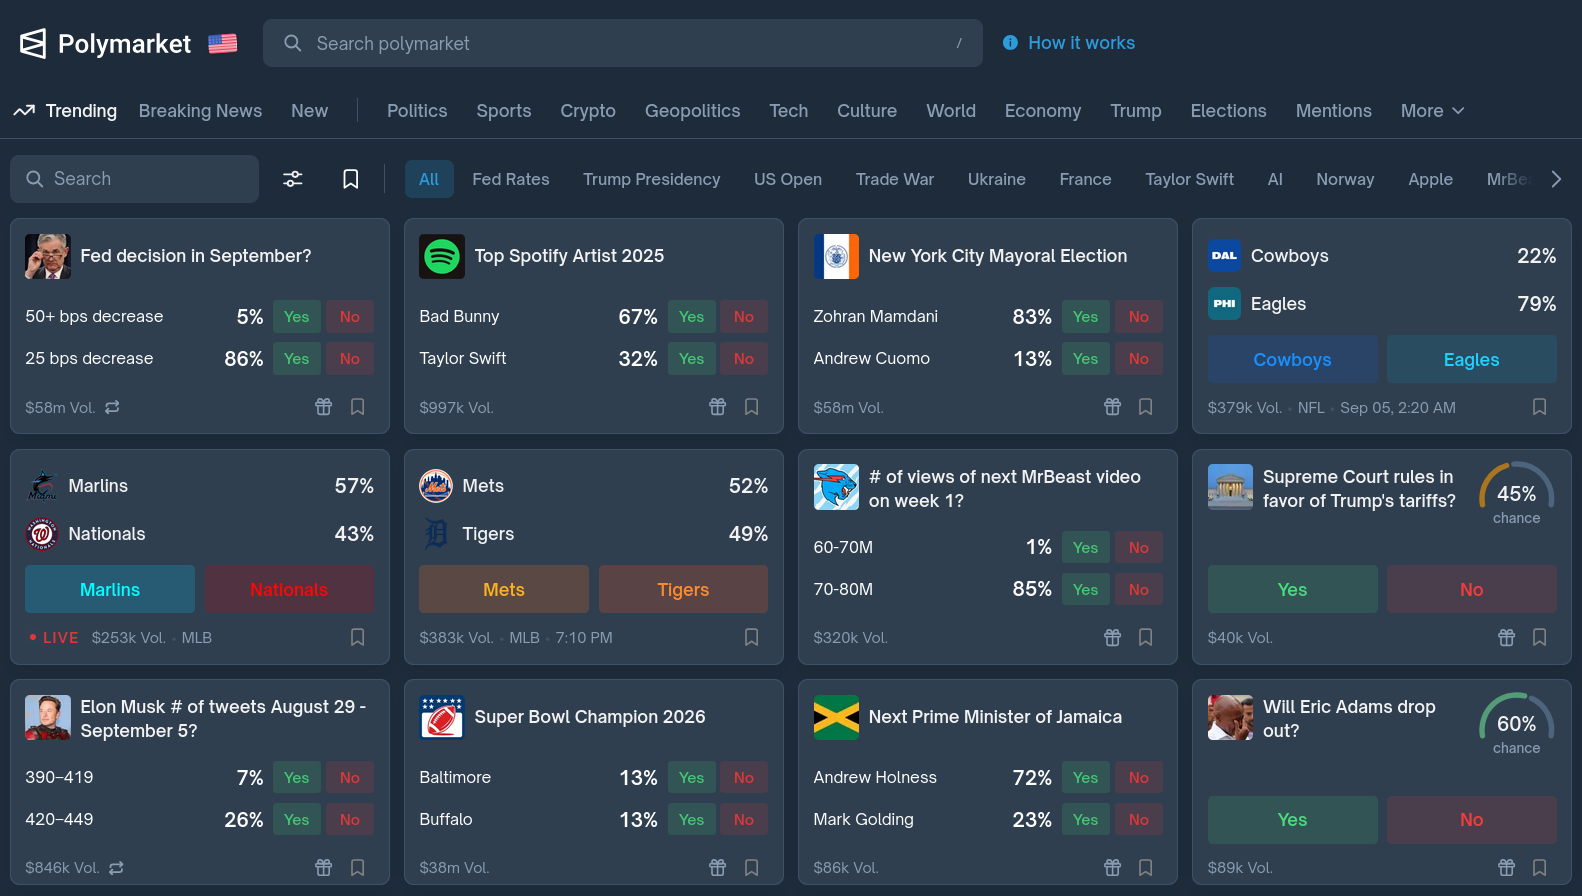
\includegraphics[width=0.95\textwidth]{figures/Polymarket_front_page.png}
  \end{center}
  \caption{The Polymarket front page as of September 3rd, 2025. While there is a variety of events, sports and politics markets are among the most popular}
  % \label{fig:front_page}
\end{figure}


On Polymarket, prediction markets are grouped into "events", which contain "markets" related to a single topic/occasion.
Each "market" is a winner-take-all market as outlined in Section \ref{sec:prediction_markets}. For each listed market, there are two complementary outcomes, labeled Yes and No with prices between \$0 and \$1.


% Figure % todo: Insert figure and reference it
% depicts the Polymarket event for the interest rate decision of the FOMC following their scheduled September meeting.

% Caption: Each market related to a possible decision (50 bps increase, 25 bps decrease, no change, etc.) related to a single FOMC meeting is grouped into 


% Figure out how to put this image where I want it to be
\begin{figure}[H]
  \begin{center}
    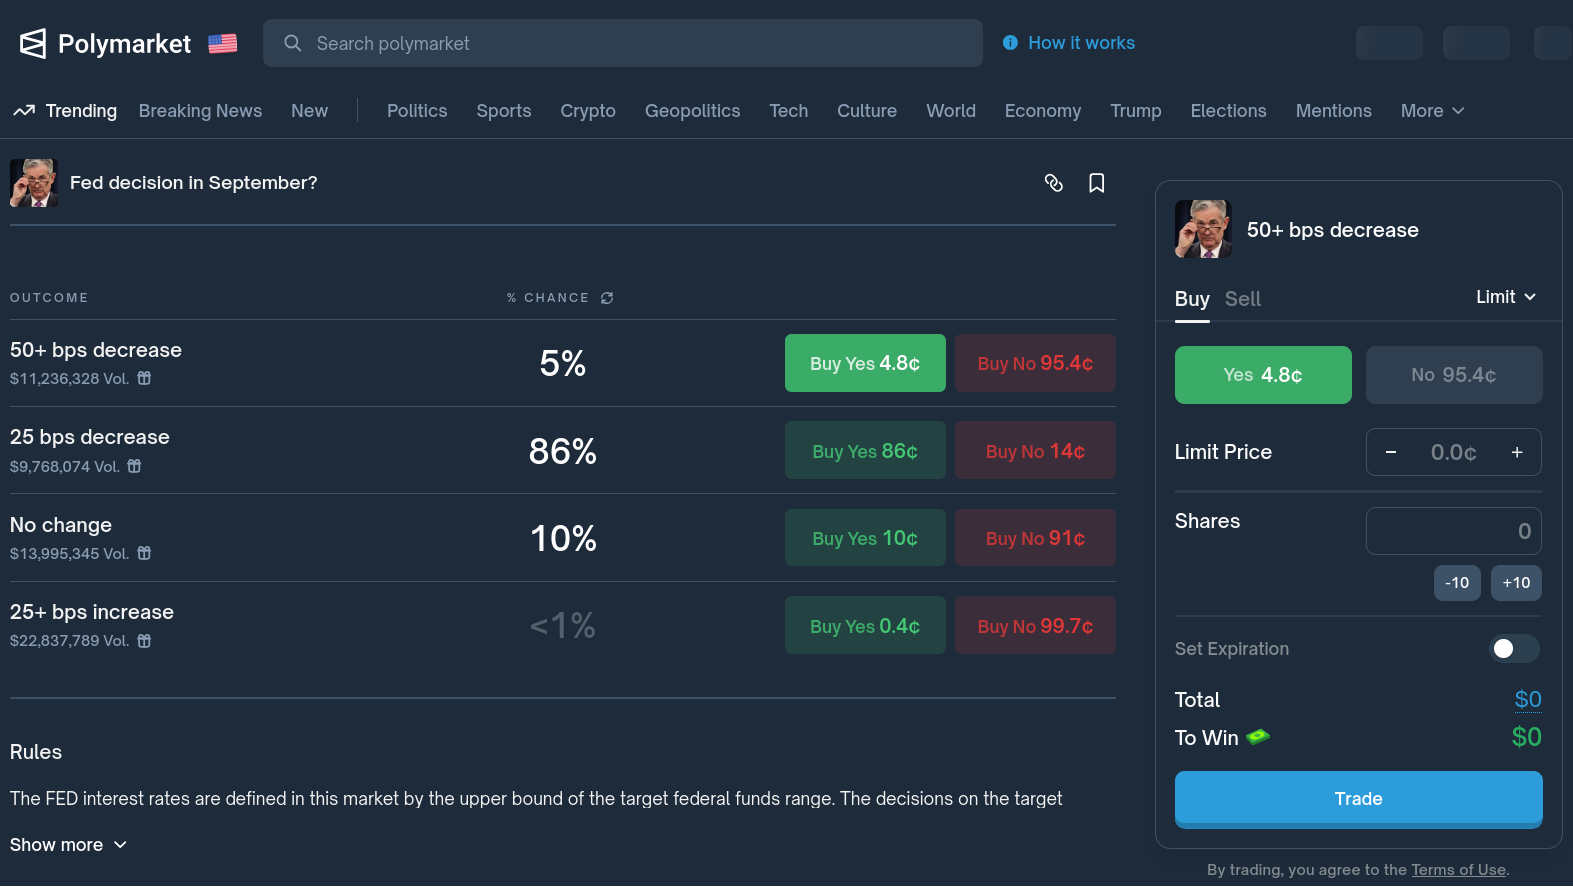
\includegraphics[width=0.95\textwidth]{figures/FOMC_event_September.png}
  \end{center}
  \caption{September FOMC event on Polymarket as of September 3rd, 2025}
  % FIX: this
  \caption*{kjansdkjnakjdnasjkdnakjdnaskjdasndjkn}
  % \label{fig:front_page}
\end{figure}


\subsubsection{design: Yes/No assets, central limit order book, and full collateralization}

%%%%%%%%%%% UNREVIEWED TEXT STARTS HERE %%%%%%%%%%%

Trading occurs on a centralized limit order book operated off-chain with on-chain settlement. Participants submit limit orders to buy or sell Yes or No claims at chosen prices; an operator matches orders and submits matched trades to an exchange smart contract that atomically swaps collateral for outcome tokens. Because the order book is continuous and open throughout the market’s life, traders can enter, exit, and revise positions at any time, and prices update in real time as new orders arrive. With two-sided liquidity, standard market microstructure logic applies: supply and demand determine the sequence of matches, and under informational efficiency, the trading process aggregates dispersed signals into prices that serve as real-time forecasts. ([Polymarket Documentation][2])

Contracts are fully collateralized at issuance and throughout trading by design. Operationally, one unit of collateral can be “split” into a full set consisting of one Yes and one No token for the same condition, ensuring that the sum of outcome shares is always backed by 1 unit of collateral that will be released to the eventual winner. Symmetrically, a holder of a full set can “merge” the tokens to reclaim collateral. At resolution, holders of the winning outcome burn their tokens to redeem the embedded collateral. This split/merge/redeem triad enforces the accounting identity behind the no-arbitrage relation $P_{\text{Yes}} + P_{\text{No}} = 1$ and guarantees performance of payoffs at resolution. ([Polymarket Documentation][3])


% Figure out how to put this image where I want it to be
\begin{figure}[H]
  \begin{center}
    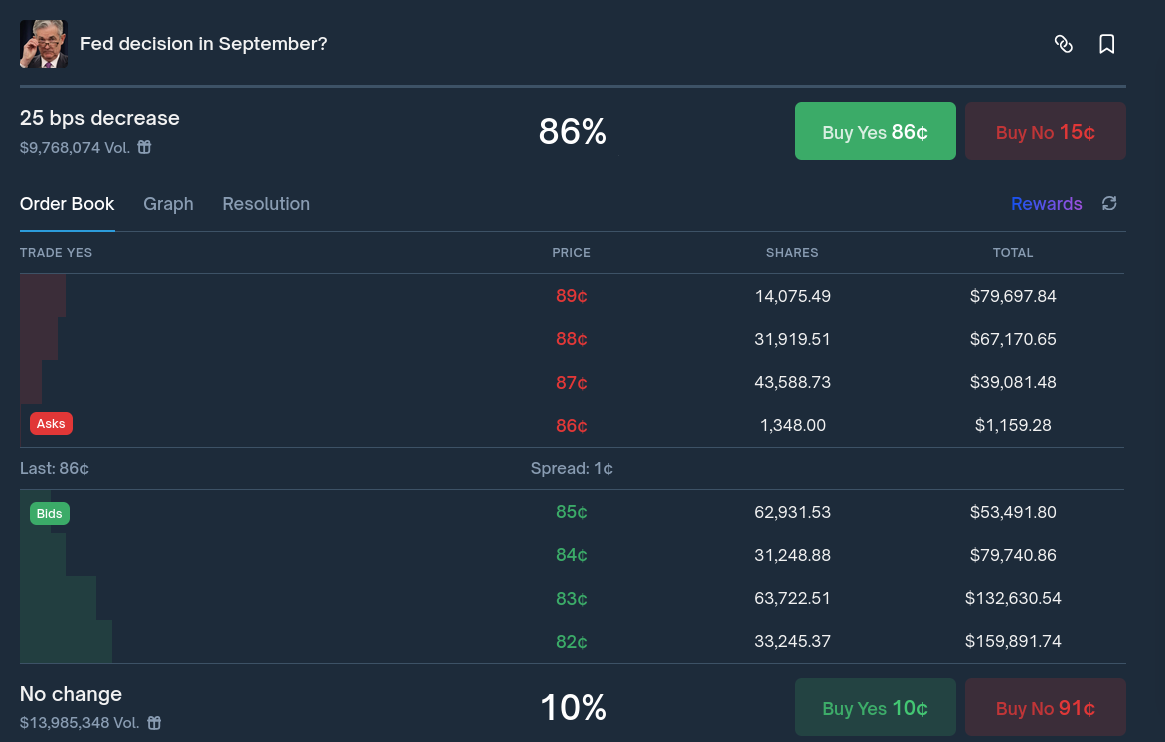
\includegraphics[width=0.95\textwidth]{figures/polymarket_continuous_double_auction.png}
  \end{center}
  \caption{The Polymarket front page as of September 3rd, 2025. While there is a variety of events, sports and politics markets are among the most popular}
  % \label{fig:front_page}
\end{figure}

\subsubsection{discovery and informational interpretation}

In this structure, each order expresses a view about mispricing of a contingent payoff. When public or private information arrives, informed traders buy underpriced outcomes or sell overpriced ones; their orders move the best quotes and, when matched, move the last trade. Under the efficient markets hypothesis, the price sequence forms a martingale with respect to the market’s information filtration, and the level of the Yes price is an efficient forecast of the event’s risk-neutral probability. The hybrid design does not change the economic logic: the off-chain order book determines matching and the on-chain settlement guarantees delivery, but the informational content is determined by competition among heterogeneous beliefs. The platform’s own presentation of prices as probabilities is consistent with this theoretical interpretation and with empirical evidence that prediction markets aggregate information effectively. ([Polymarket Documentation][4])

\subsubsection{matching mechanics and the linkage between Yes and No}

Beyond standard maker–taker matches in a single line of the book, Polymarket’s exchange contract implements order-level logic that ties the two complementary tokens together so the full-set accounting holds at execution. As documented by Saguillo, Ghafouri, Kiffer and Suarez-Tangil (2025), there are three economically distinct pathways by which orders get matched and settled:

Direct trade. A taker’s marketable limit order in a given outcome token matches resting maker orders on the same side of the market. Settlement is a straightforward token-for-collateral swap at the matched price(s). On-chain, these fills are recorded as OrderFilled events. This is the pure order-book mechanism familiar from equities, and it governs most routine executions. ([arXiv][5])

Mint via PositionSplit. Because complementary outcomes must sum to one dollar of collateral, the exchange can also satisfy opposite-side demand across the two books by minting a new full set. When a buy order for Yes at price $p$ meets a buy order for No at price $1-p$, the contract locks 1 unit of collateral and mints one Yes and one No token, delivering each to the respective buyer. Economically, this is equivalent to sourcing inventory from the collateral pool rather than from an external holder. On-chain, the mint is captured by a PositionSplit event alongside OrderFilled events for the two sides. This pathway helps keep the two order books coupled and supports tight complementary pricing even when inventory on one side is scarce. ([arXiv][5], [Polymarket Documentation][3])

Burn via OrdersMerged. The reverse operation retires a full set and releases collateral when aggregate sell orders across the two books sum to one dollar. For example, simultaneous sells of Yes at $p$ and No at $1-p$ allow the contract to burn the pair of tokens and return 1 unit of collateral to the sellers’ counterparties, recording an OrdersMerged event together with the corresponding OrderFilled events. Economically, this drains inventory back into the collateral pool and enforces the accounting constraint in the face of two-sided liquidation pressure. ([arXiv][5], [Polymarket Documentation][6])

These three execution paths are complementary: the direct trade path matches inventory held by other users; the PositionSplit path manufactures fresh inventory when demand is balanced across the complementary books; and the OrdersMerged path retires inventory when supply is balanced. Each path preserves the invariant that a Yes and a No for the same condition are worth, in combination, exactly one unit of collateral at issuance and prior to resolution. The platform’s order-book and API documentation reflect the maker–taker structure and the unified handling of complementary tokens, while independent data sources expose these mechanics through emitted events such as OrdersMatched at the taker level and OrderFilled/OrdersMerged at settlement. ([Polymarket Documentation][2], [Goldsky][7])

\subsubsection{inventory transformations and their implications}

Crucially, the split/merge operations are not restricted to matching engine internals; users may proactively split collateral into a full set or merge a full set back into collateral at any time after a condition is prepared. This enables inventory management and hedging strategies familiar from contingent-claim markets. A trader who wants to make a market can mint full sets to provision inventory on both sides; a trader who has accumulated offsetting Yes and No across executions can merge to crystallize collateral and compress balance-sheet usage. At the microstructure level, these user-driven transformations add elasticity to supply on both sides of the book, which, in turn, tightens complementary pricing and facilitates efficient price discovery. In combination with the three settlement pathways, they make explicit the tight coupling between the books for Yes and No and operationalize the economic identity that one unit of collateral underlies the pair. ([Polymarket Documentation][3])

\subsubsection{and redemption}

% Put this where redemption is explained


% September market rules
\begin{quote}
  {
    \raggedright
    The FED interest rates are defined in this market by the upper bound of the target federal funds range. The decisions on the target federal fund range are made by the Federal Open Market Committee (FOMC) meetings.

    This market will resolve to the amount of basis points the upper bound of the target federal funds rate is changed by versus the level it was prior to the Federal Reserve's September 2025 meeting.

    If the target federal funds rate is changed to a level not expressed in the displayed options, the change will be rounded up to the nearest 25 and will resolve to the relevant bracket. (e.g. if there's a cut/increase of 12.5 bps it will be considered to be 25 bps)

    The resolution source for this market is the FOMC’s statement after its meeting scheduled for September 16 - 17, 2025 according to the official calendar:
    % \linebreak
    https://www.federalreserve.gov/monetarypolicy/fomccalendars.htm.

    The level and change of the target federal funds rate is also published at the official website of the Federal Reserve at
    % \linebreak
    https://www.federalreserve.gov/monetarypolicy/openmarket.htm.

    This market may resolve as soon as the FOMC’s statement for their September meeting with relevant data is issued. If no statement is released by the end date of the next scheduled meeting, this market will resolve to the "No change" bracket. 
  }
\end{quote}

When the designated oracle finalizes the event’s outcome, the winning side is set to a payout of 1 while the losing side’s payout is 0. Holders of the winning token redeem by burning their positions for collateral via the contract’s redeem function. Because the system remained fully collateralized ex ante, there is no gap risk at resolution; the accounting identity closes as collateral is released to the winner and all losing tokens expire. This completes the contingent-claim lifecycle from issuance, through trading and inventory transformations, to settlement and redemption. ([Polymarket Documentation][8])


%%%%%%%%%%% UNREVIEWED TEXT ENDS HERE %%%%%%%%%%%





% TODO: Humanise
\subsection{Polymarket}



% \subsubsection{claims and probabilistic pricing}
%
%
% ## Summary
%
% Polymarket can be read entirely through the lens of contingent-claim pricing and order-driven microstructure. Yes and No outcome claims are fully collateralized complements whose prices add to one and whose Yes price is the market’s risk-neutral probability of the event. A hybrid CLOB matches orders continuously, with three settlement pathways-direct trade, mint via PositionSplit, and burn via OrdersMerged—tying the complementary books together. Users themselves can split and merge full sets, adding supply elasticity and aiding price alignment. Under standard efficiency assumptions, this design delivers real-time price discovery in the form of probability-like prices that aggregate dispersed information about future events. ([Polymarket Documentation][2], [arXiv][5])
%
% [1]: https://docs.polymarket.com/polymarket-learn/FAQ/what-are-prediction-markets?utm_source=chatgpt.com "What is a Prediction Market?"
% [2]: https://docs.polymarket.com/developers/CLOB/introduction?utm_source=chatgpt.com "CLOB Introduction"
% [3]: https://docs.polymarket.com/developers/CTF/split?utm_source=chatgpt.com "Splitting USDC"
% [4]: https://docs.polymarket.com/polymarket-learn/trading/how-are-prices-calculated?utm_source=chatgpt.com "How Are Prices Calculated?"
% [5]: https://arxiv.org/html/2508.03474v1 "Unravelling the Probabilistic Forest: Arbitrage in Prediction Markets"
% [6]: https://docs.polymarket.com/developers/CTF/merge?utm_source=chatgpt.com "Merging Tokens"
% [7]: https://goldsky.com/blog/polymarket-dataset?utm_source=chatgpt.com "Announcing: Polymarket Datasets Available Now - Goldsky"
% [8]: https://docs.polymarket.com/developers/CTF/redeem?utm_source=chatgpt.com "Reedeeming Tokens"


% TODO: Humanise
\subsection{Federal Funds Rate futures}

\subsubsection{Effective Federal Funds Rate (EFFR)}

The effective federal funds rate is the transaction-volume-weighted median interest rate on unsecured overnight loans of reserve balances between depository institutions in the United States. The Federal Reserve Bank of New York computes the EFFR from FR 2420 transactional reports and publishes it for the prior business day at approximately 9:00 a.m. New York time. This benchmark rate is the underlying reference for CME’s 30-Day Federal Funds futures.
% TODO: Add citation for fed article describing EFFR
% \cite{FED OF New York}

\subsubsection{Price quoting and the implied monthly average}

CME 30-Day Federal Funds (ZQ) futures are quoted in IMM index terms, with price equal to 100 minus the market-implied arithmetic average of daily EFFR over the contract’s calendar month. If the futures price for month T is $P_t^T$ (percent), the implied expected monthly average is

$$\mathbb{E}_t[\overline{r}_T] = 100 - P_t^T$$

where $\overline{r}_T$ denotes the arithmetic average of daily EFFR realizations during month $T$. This mapping follows directly from the contract’s price quotation and settlement definition. 
% TODO: add citation for CME group's FedWatch methodology tool


\subsubsection{High-level assumptions for extracting probabilities}

To translate ZQ prices into probabilities of FOMC outcomes, the CME FedWatch methodology adopts three core assumptions.

First, rate changes occur in uniform 25-basis-point increments and the EFFR adjusts proportionally to the target change.

Second, within a meeting month, the EFFR is piecewise constant: it equals a pre-meeting level up to the decision’s effective date, and a post-meeting level thereafter.

Third, anchor months without FOMC meetings pin down a month-end/start-of-next-month level that is used to propagate boundary conditions through adjacent months. Under these assumptions, ZQ prices encode a risk-neutral expectation of the path of EFFR that can be decomposed into before/after segments in meeting months and rolled across months via anchors.
% TODO: add citation for CME group's FedWatch methodology tool

\subsubsection{Anchor months and boundary conditions}

In any month with no scheduled FOMC meeting, the entire calendar month is governed by a single policy regime, so the ZQ-implied average equals the expected EFFR throughout the month. FedWatch uses these months as anchors: for an anchor month $T$,

$$\text{EFFR(End)}_{T-1}=\text{EFFR(Avg)}_{T}=\text{EFFR(Start)}_{T+1}$$

Operationally, one identifies the nearest full non-meeting month, reads $\text{EFFR(Avg)}_{T}=100-P^T$ from its ZQ price, sets the end of the prior month and the start of the following month to that level, and then propagates these boundary values backward and forward as needed when solving adjacent meeting months. This anchoring step provides the initial conditions for the system of month-by-month equations.
% TODO: add citation for CME group's FedWatch methodology tool

\subsubsection{Meeting months and the time-weighting identity}

Consider a meeting month $T$ with $m_T$ calendar days and $k_T$ days before the policy change becomes effective. Let $r_T^{-}$ denote the pre-meeting EFFR level and $r_T^{+}$ the post-meeting level. Because the futures price reflects the arithmetic monthly average, the implied average satisfies the time-weighting identity

$$\mathbb{E}_t[\overline{r}_T] = \omega_T\, r_T^{-} + (1-\omega_T)\,\mathbb{E}_t[r_T^{+}], \qquad \omega_T \equiv \frac{k_T}{m_T}
$$

Solving for the expected post-meeting level gives

$$\mathbb{E}_t[r_T^{+}] = \frac{m_T\,\mathbb{E}_t[\overline{r}_T] - k_T\, r_T^{-}}{m_T-k_T}$$

When the following month $T{+}1$ is an anchor, $\mathbb{E}_t[r_T^{+}]$ is identified directly from $\text{EFFR(Avg)}_{T+1}$. On the other hand, if the prior month is an anchor, $\,r_T^{-}$ is identified from $\text{EFFR(Avg)}_{T-1}$. In either case, the time-weighting identity links the observable ZQ-implied monthly average to the unobservable post-meeting level and enables sequential solution across the term structure. 
% TODO: add citation for CME group's FedWatch methodology tool

\subsubsection{Probability calculations via the characteristic–mantissa method}

Define the expected change in EFFR over the meeting month as $\Delta_T^{*} \equiv \mathbb{E}_t[r_T^{+}] - r_T^{-}$. Express this in units of 25 bps, $\,n_T^{*} \equiv \Delta_T^{*}/0.25\%$. Decompose $n_T^{*}$ into its characteristic (integer) and mantissa (fractional) parts:

$$
n_T^{*} = n_T + y_T,\qquad n_T \in \mathbb{Z}_{\ge 0}, 0 \le y_T < 1.
$$

FedWatch interprets this as two mutually exclusive outcomes at the meeting: a change of $n_T \times 25$ bps with probability $1-y_T$, and a change of $(n_T{+}1)\times 25$ bps with probability $y_T$. When the expected change is less than one increment ($n_T=0$), this reduces to the familiar binomial case of no change versus a single 25-bp move with probabilities $1-y_T$ and $y_T$, respectively. In the special case where the next month is an anchor and one wishes to ask only “hike or hold by 25 bps,” the implied probability collapses to

$$
\mathbb{P}(\text{25 bp hike}) 
= \frac{\text{EFFR(End)}_{T}-\text{EFFR(Start)}_{T}}{0.25\%},
\qquad 
\mathbb{P}(\text{hold})=1-\mathbb{P}(\text{hike}),
$$

